% Präambel
\documentclass[12pt,a4paper,oneside, 
liststotoc, 					% Tabellen- und Abbildungsverzeichnis ins Inhaltsverzeichnis
bibtotoc,						% Literaturverzeichnis ins Inhaltsverzeichnis aufnehmen
titlepage, 						% Titlepage-Umgebung statt \maketitle
headsepline, 					% horizontale Linie unter Kolumnentitel
%abstracton,					% Überschrift beim Abstract einschalten, Abstract muss dazu in {abstract}-Umgebung stehen
%DIV11,							% auskommentieren, um den Seitenspiegel zu vergrößern
BCOR=6mm,						% Bindekorrektur, die den Seitenspiegel um 6mm nach rechts verschiebt,
]{scrreprt}			
\usepackage{ucs} 				% Dokument in utf8-Codierung schreiben und speichern
\usepackage[utf8x]{inputenc} 	% ermöglicht die direkte Eingabe von Umlauten
\usepackage[ngerman]{babel} 	% deutsche Trennungsregeln und Übersetzung der festcodierten Überschriften
\usepackage[T1]{fontenc} 		% Ausgabe aller zeichen in einer T1-Codierung (wichtig für die Ausgabe von Umlauten!)
\usepackage{graphicx}  			% Einbinden von Grafiken erlauben
\usepackage{caption}
%\usepackage{amsmath}
%\usepackage{amsfonts}
%\usepackage{amssymb}
\usepackage{mathpazo} 			% Einstellung der verwendeten Schriftarten
\usepackage{textcomp} 			% zum Einsatz von Eurozeichen u. a. Symbolen
\usepackage{listings}			% Datstellung von Quellcode mit den Umgebungen {lstlisting}, \lstinline und \lstinputlisting
\usepackage{xcolor} 			% einfache Verwendung von Farben in nahezu allen Farbmodellen
\usepackage{url, hyphenat}
\usepackage[intoc]{nomencl} 	% zur Erstellung des Abkürzungsberzeichnisses
\usepackage{fancyhdr}			% Zusatzpaket zur Gestaltung von Fuß und Kopfzeilen
\usepackage{setspace}
\usepackage[export]{adjustbox}
\usepackage[numbers, sort]{natbib}
\usepackage{pdfpages}
\usepackage{float}
\usepackage{lmodern}
\usepackage{dirtree}

% -----------------------------------------------------------------------------------------------------------------
% Zum Aktualisieren des Abkürzungsverzeichnisses bitte auf der Kommandozeile folgenden Befehl aufrufen :
%  makeindex Bachelorarbeit.nlo -s nomencl.ist -o Bachelorarbeit.nls
% -----------------------------------------------------------------------------------------------------------------

% Hier die persönlichen Daten eingeben:

\newcommand{\untertitel}{Stauerkennung auf Autobahnwebcam-Bildern mit geringer Ressourcenverwendung}
\newcommand{\arbeit}{Studienarbeit}
\newcommand{\studiengang}{Angewandte Informatik}
\newcommand{\autor}{Maurice Heumann \& Mirko Müller}
\newcommand{\matrikelnr}{3970752 \& 8...}
\newcommand{\kurs}{TINF16B4}
\newcommand{\firma}{CAS Software AG}
\newcommand{\abgabe}{17. September 2018}
\newcommand{\betreuerfirma}{Dr. Christian Bomhardt}

\newcommand{\jahr}{2018}			% für Angabe im Copyright-Vermerk der Titelseite

% Abkürzungen
\newcommand{\ua}{\mbox{u.\,a.\ }}
\newcommand{\oae}{\mbox{o.\,Ä.\ }}
\newcommand{\zB}{\mbox{z.\,B.\ }}
\newcommand{\bs}{$\backslash$}

\renewcommand{\nomname}{Abkürzungsverzeichnis}
\newcommand{\source}[2]{\caption*{\centering \footnotesize Quelle: \url{#1} ({#2})}}

\definecolor{blub}{rgb}{0.1, 0.1, 0.1}
\newcommand{\dirheader}[1]{{#1}}
\newcommand{\dirfile}[1]{\textit{#1}}

\newcommand{\*}{\newline}

% ------------------------
\usepackage[pdftex,
            pdfauthor={\autor},
            pdftitle={\untertitel},
            %pdfsubject={The Subject},
            %pdfkeywords={Some Keywords},
            %pdfproducer={Latex with hyperref, or other system},
            %pdfcreator={pdflatex, or other tool}
						]{hyperref}

% -------------------------------------------------------------------------------------------
% Definition der Kopf- und Fußzeilen
\lhead{}								% Kopf links
\chead{}								% Kopf mitte
\rhead{\sffamily{\autor}}								% Kopf rechts
\lfoot{}								% Fuß links
\cfoot{\sffamily{\thepage}}			% Fuß mitte
\rfoot{}				% Fuß rechts
\renewcommand{\headrulewidth}{0.4pt}	% Liniendicke Kopf
\renewcommand{\footrulewidth}{0.4pt}	% Liniendicke Fuß

\makenomenclature							% Abkürzungsverzeichnis erstellen

% alle Abkürzungen, die in der Bachelorarbeit verwendet werden

\nomenclature{DHBW}{Duale Hochschule Baden-Württemberg}
\nomenclature{UI}{User Interface}
\nomenclature{API}{Application Programming Interface}
\nomenclature{HTTP}{Hypertext Transfer Protocol}
\nomenclature{HTTPS}{Hypertext Transfer Protocol Secure}
\nomenclature{SSL}{Secure Sockets Layer}
\nomenclature{SVZ}{Straßenverkehrszentrale}
\nomenclature{PNG}{Portable Network Graphics}
\nomenclature{JSON}{JavaScript Object Notation}
\nomenclature{TLS}{Transport Layer Security}
\nomenclature{SQL}{Structured Query Language}
\nomenclature{JPEG}{Joint Photographic Experts Group}
					% Datei mit Abkürzungen laden

% -------------------------------------------------------------------------------------------
%                     Beginn des Dokumenteninhalts
% -------------------------------------------------------------------------------------------
\begin{document}
\setcounter{secnumdepth}{3}					% Nummerierungstiefe fürs Inhaltsverzeichnis
\setcounter{tocdepth}{3}
\sffamily									% für die Titelei serifenlose Schrift verwenden

% ------------------------------ Titelei -----------------------------------------------------

\thispagestyle{plain}
\begin{titlepage}
\enlargethispage{4.0cm}
\sffamily 								% Serifenlose Grundschrift für die Titelseite einstellen
	


\includegraphics[height=2cm]{Bilder/cas.png}
\hfill

\includegraphics[height=1.3cm]{Bilder/dhbw.png}
\vspace*{2.0cm}
\begin{center}

\Large{\textbf{\untertitel}}\\[5ex]
\LARGE{\textbf{\arbeit}}\\[2ex]
\normalsize{für die Prüfung zum\\[1ex] Bachelor of Science}\\[3ex]
\Large{Studiengang \studiengang}\\[1ex]
\normalsize{Duale Hochschule Baden-Württemberg Karlsruhe}\\[5ex]
von\\[1ex] \autor \\[18ex]


\begin{tabular}{ll}
Abgabedatum:                   & \quad \abgabe \\
Matrikelnummer:                & \quad \matrikelnr \\ 
Kurs:                          & \quad \kurs \\ 
Ausbildungsfirma:              & \quad \firma \\ 
Betreuer der Ausbildungsfirma: & \quad \betreuerfirma \\ [5ex]

\end{tabular}
\end{center} 
\end{titlepage} 				% erzeugt die Titelseite
\pagenumbering{Roman}						% große, römische Seitenzahlen für Titelei
\addchap{Eidesstattliche Erklärung}
Erklärung gemäß § 5 (3) der ”Studien- und Prüfungsordnung DHBW Technik“ vom 22. September 2011.\\
\\
Ich versichere hiermit, dass ich die vorliegende Arbeit selbständig verfasst und keine anderen als die angegebenen Quellen und Hilfsmittel benutzt habe.\\
%\\
%Ich versichere zudem, dass die eingereichte elektronische Fassung mit der gedruckten Fassung
%übereinstimmt.\\[10ex]

Karlsruhe, den \today \\[4ex]


\rule[-0.2cm]{5cm}{0.5pt} \\

\textsc{\autor} \\[10ex]

\hrule 
\vspace*{1.0cm}
\noindent \textbf{\Large{Sperrvermerk}}\\
\normalsize
Die Ergebnisse der Arbeit stehen ausschließlich dem auf dem Deckblatt aufgeführten Ausbildungsbetrieb zur Verfügung.

\vspace*{1.0cm}
\noindent \textbf{\Large{Copyrightvermerk}}\\
\normalsize
Dieses Werk einschließlich seiner Teile ist \textbf{urheberrechtlich geschützt}. Jede Verwertung außerhalb der engen Grenzen des Urheberrechtgesetzes ist ohne Zustimmung des Autors unzulässig und strafbar. Das gilt insbesondere für Vervielfältigungen, Übersetzungen, Mikroverfilmungen sowie die Einspeicherung und Verarbeitung in elektronischen Systemen.
\begin{flushright}
\copyright{} \jahr
\end{flushright} 				% Einbinden der eidestattlichen Erklärung
\chapter*{Abstract} %*-Variante sorgt dafür, das Abstract nicht im Inhaltsverzeichnis auftaucht
Das ist ein Abstract.   				% Einbinden des Abstracts

\tableofcontents							% Erzeugen des Inhalsverzeichnisses
\printnomenclature[2.0cm]					% Erzeugen des Abkürzungsverzeichnisses
\listoffigures 								% Erzeugen des Abbildungsverzeichnisses 
%\listoftables 								% Erzeugen des Tabellenverzeichnisses
\pagebreak

% --------------------------------------------------------------------------------------------
%                    Inhalt der Bachelorarbeit
%---------------------------------------------------------------------------------------------
\pagenumbering{arabic}						% arabische Seitenzahlen für den Hauptteil
\pagestyle{fancy}				
\onehalfspacing
\rmfamily

\renewcommand{\lstlistingname}{Quelltext}

\lstdefinelanguage{JavaScript}{
  keywords={typeof, new, true, false, catch, function, return, null, catch, switch, var, if, in, while, do, else, case, break},
  keywordstyle=\color{blue}\bfseries,
  ndkeywords={class, export, boolean, throw, implements, import, this},
  ndkeywordstyle=\color{darkgray}\bfseries,
  identifierstyle=\color{black},
  sensitive=false,
  comment=[l]{//},
  morecomment=[s]{/*}{*/},
  commentstyle=\color{purple}\ttfamily,
  stringstyle=\color{red}\ttfamily,
  morestring=[b]',
  morestring=[b]"
}

\lstdefinelanguage{CSS} {
	morekeywords={color,background,margin,padding,font,weight,display,position,top,left,right,bottom,list,style,border,size,white,space,min,max-width,width}, 
	sensitive=false, 
	morecomment=[l]{//}, 
	morecomment=[s]{/*}{*/}, 
	morestring=[b]", 
} 

\lstset{
  breakatwhitespace=false,
  breaklines=true,
  captionpos=b,
  extendedchars=true,
  keepspaces=true,
  language=Java,
  showspaces=false,
  showstringspaces=false,
  showtabs=false,
  tabsize=2,
	frame=lines,
	basicstyle=\footnotesize\ttfamily,
	backgroundcolor=\color{white},
	keywordstyle=\color{blue},
  commentstyle=\color{green!40!black},
  %identifierstyle=\color{blue},
  stringstyle=\color{orange}
}

\sloppy
\chapter{Einleitung}
\label{cha:Einleitung}
* Stauanalyse anhand von Verkehrskameras
* Geringe Ressourcenverwendung

\section{Motivation}
\label{sec:Motivation}
* Arbeitsweg über A5
* Oft Stau
* Google / Radio oftmals nicht schnell genug, gerade morgens
* Verkehrskameras meist max. 1 Minute im Verzug
* Aktuell genug um Analyse des Verkehrs durchzuführen
* Bei zu viel Verkehr alternative Route wählen

\section{Ziel der Arbeit}
\label{sec:ZielDerArbeit}
* Android App
* Erkennen des Verkehrszustandes anhand von Verkehrskameras der SVZ-BW
* Analyse der Route und Vorschlagen einer Alternativroute (Ausfahrtmöglichkeit aufzeigen)
* Auf Arbeit des letzten Jahrgangs aufbauen
* Neuronales Netz zu Ressourcenintensiv, um aktiv zu betreiben
* Möglichst geringe Ressourcen
* Geringe Serverlast sofern möglich
* Geringe Handylast -> geringer Akkuverbrauch
* Ziel also ausgewogene Lösung finden, die Stau gut (nicht zwangsläufig optimal) erkennt, aber dafür guten
	Ressourcenverbrauch hat und einsetzbar ist
\chapter{Grundlagen}

Dieses Kapitel beschreibt Grundlagen, die für das weitere Verständnis der Arbeit benötigt werden.

\section{Straßenverkehrszentrum Baden-Württemberg} % Mi

\section{Histogramm} % Mi

\section{Faltungskerne} % Mo
Faltungskerne beschreiben Filter in der Bildverarbeitung, die über die diskrete Faltung im 2-dimensionalen
Raum auf ein Bild angewendet werden.


Grundsätzlich ist die 1-dimensionale Faltung im kontinuierlichen Raum definiert durch die Integration zweier Funktionen {\em g} und {\em f} an einem Punkt {\em t}, wobei die Funktion {\em g} gespiegelt wird, also auf {\em f} gefaltet wird:

$$ (f * g)(t) = \int_{-\infty}^{\infty} f(\tau)g(t - \tau) d\tau $$

Für die Bildverarbeitung ist jedoch die Faltung im kontinuierlichen 2-dimensionalen Raum relevant.
Hierfür wird statt dem Integral, die Doppelsumme über alle Werte {\em n} gebildet (in {\em x}- und {\em y}-Richtung) und der Filter {\em k} mit dem Bild {\em I} an einem Punkt {\em (x, y)} gefaltet:

$$ I\mbox{*}(x, y) = \sum_{i=1}^{n}\sum_{j=1}^{n} I(x - i, y - j)k(i, j) $$

Hiermit wird nun eine Faltungsmatrix, bzw. ein Faltungskern auf jeden Pixel im Bild angewendet:

$$ k = \left( \begin{array}{rrr}
1 & 1 & 1 \\
1 & 1 & 1 \\
1 & 1 & 1 \\
\end{array}\right) $$

Faltungskerne sind lokale Operatoren, die die Neuberechnung eines Pixels mittels eines Teilbereichs des Bildes durchführen.
Mit solchen Filtern lassen sich Bilder beispielsweise Schärfen, Glätten. Es lassen sich jedoch auch Kanten finden oder Rauschanteile reduzieren.

\subsection{Gauß-Filter}
Der Gauß-Filter ist ein Faltungskern, welcher über eine gaußsche Glockenkurve gebildet wird.
Mit solch einem Filter lassen sich Bilder glätten und somit Rauschanteile reduzieren.
Bilder wirken dadurch weicher, bzw. verwaschen.

Ein möglicher Faltungskern sähe so aus:

$$ \frac{1}{16} \left( \begin{array}{rrr}
1 & 2 & 1 \\
2 & 4 & 2 \\
1 & 2 & 1 \\
\end{array}\right) $$

Wendet man diesen Filter auf ein Bild mit der diskreten Faltung an, erhält man dieses Ergebnis:

\begin{figure}[ht]
   \centering
     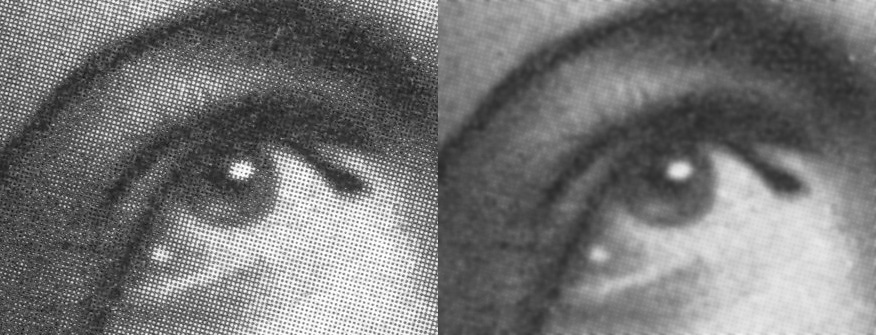
\includegraphics[width=11cm]{Bilder/Gaussian_Blur} \\
 \caption{Anwendung eines Weichzeichnungsfilters}
 \source{https://de.wikipedia.org/wiki/Datei:Halftone,_Gaussian_Blur.jpg}{10.3.2019}
 \label{fig:Blur}
\end{figure}

\subsection{Laplace-Filter}
Ein Laplace-Filter ist ein Faltungskern zur Kantendetektion innerhalb eines Bildes.
Unter einer Kante versteht man hierbei eine rasche Veränderung der Helligkeitswerte entlang einer Richtung.

Um Kanten zu finden wird ein Operator auf das Bild angewendet, welcher die zweite Ableitung bildet (Laplace-Operator). Abrupte Schwankungen der Intensitätswerte werden dadurch als Nulldurchgänge sichtbar.

Über die Faltung des Operators der Vorwärtsdiffenz {\em (1 -1)} mit sich selbst, lässt sich ein 1-dimensionaler Faltungskern der zweiten Ableitung bilden: {\em (1 -2 1)}.
Dieser Kern lässt sich transponieren, um ein Bild nicht nur in x-, sondern auch in y-Richtung abzuleiten.
Beide Kerne kombiniert ergeben den Laplace-Filter:

$$ \left( \begin{array}{rrr}
0 & 1 & 0 \\
1 & -4 & 1 \\
0 & 1 & 0 \\
\end{array}\right) $$

Wendet man diesen Filter auf ein Bild an, erhält man folgendes Ergebnis:

\begin{figure}[ht]
   \centering
     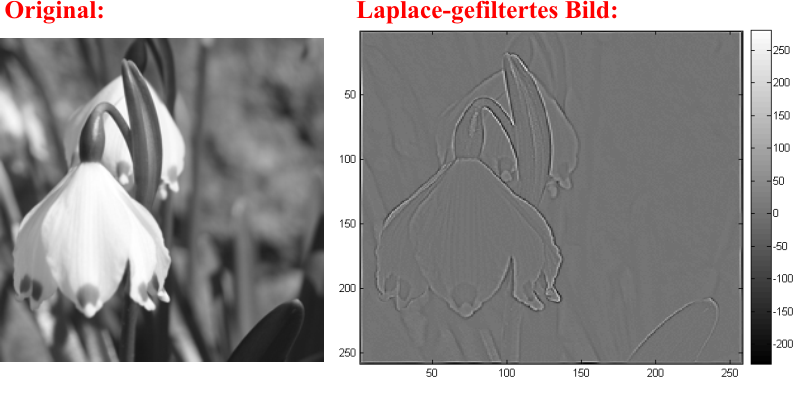
\includegraphics[width=11cm]{Bilder/Laplace} \\
 \caption{Anwendung eines Laplace-Filters}
 \source{https://de.wikipedia.org/wiki/Datei:Laplace_beispiel.png}{10.3.2019}
 \label{fig:Laplace}
\end{figure}

Aufgrund eines hohen Rauschanteils in natürlichen Bildern liefert dieser Filter jedoch nicht immer gute Resultate.

\subsection{Sobel-Operator}
Um auf natürlichen Bildern Kanten zuverlässig zu erkennen, kombiniert der Sobel-Operator die Ideen des Gauß- und Laplace-Filters.
Hierbei wird das Bild in eine Richtung über die zentrale Differenz {\em (1 0 -1)} abgeleitet, andere Richtung jedoch über einen Gauß-Filter {\em (1 2 1)} geglättet,
um Rauschanteile zu reduzieren.
Kombiniert man beide Filter miteinander, erhält man den Sobel-Operator

$$ \left( \begin{array}{rrr}
-1 & 0 & 1 \\
-2 & 0 & 2 \\
-1 & 0 & 1 \\
\end{array}\right) $$

Dadurch werden Kanten jedoch nur in eine Richtung erkannt.
Um Kanten in die jeweils andere Richtung zu erkennen, kann die Faltungsmatrix transponiert werden und ebenfalls auf
das Ausgangsbild angewendet werden.

Die beiden erhaltenen Ergebnisse können nun vereint werden, um alle Kanten innerhalb eines Bildes zu erhalten:

\begin{figure}[ht]
   \centering
     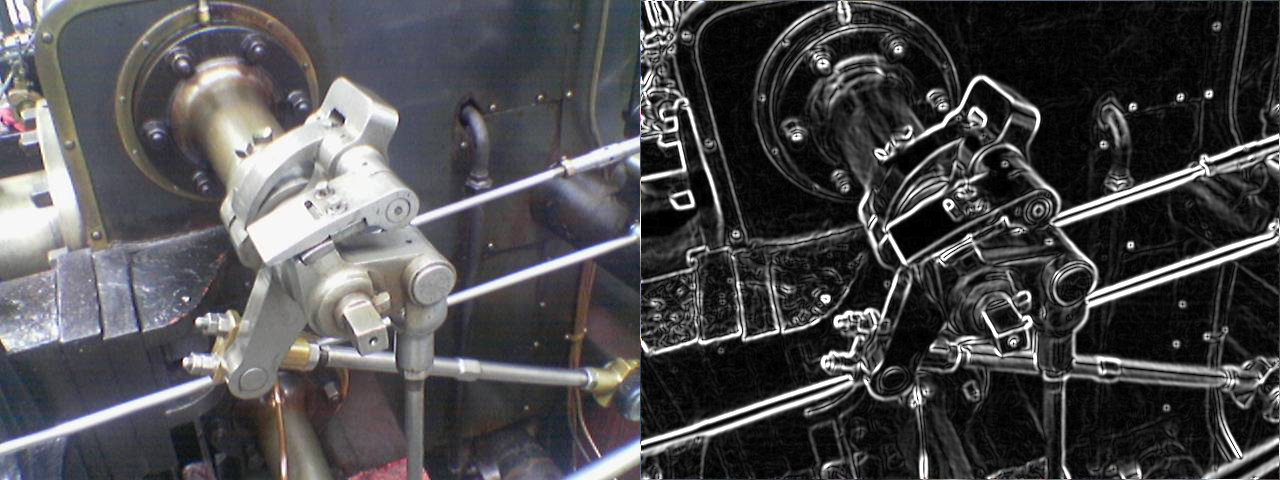
\includegraphics[width=11cm]{Bilder/Sobel} \\
 \caption{Anwendung eines Sobel-Operators}
 \source{https://en.wikipedia.org/wiki/File:Valve_sobel_(3).PNG}{10.3.2019}
 \label{fig:Sobel}
\end{figure}

\section{Canny-Edge-Detection} % Mi
\section{Otsu} % Mi
\section{Haar-Features} % Mi

\section{Morphologische Operatoren} % Mo
\subsection{Erosion}
\subsection{Dilatation}
\subsection{Closing}
\subsection{Opening}

\section{OpenCV} % Mi

\chapter{Hauptteil}
\chapter{Zusammenfassung}

% Kritische, inhaltliche Reflexion von Theorie und Praxis 
\section{Fazit}
*Optimierter Algorithmus und optimierte Implementierung\newline
*Effizenz vs Genauigkeit\newline
*weniger dynamisch als mashine learning\newline
*

\section{Ausblick}
*Besseres Background-Model?\newline
*Mehr Vor-/Nach-Verarbeitung?\newline
*Genauere/Automatische Schwellwerte?\newline
*Alternative Datenquelle finden?\newline
*Mehr Features (Ausfahrten erkennung, Entfernung zur Ausfahrt)\newline
*Mehr UI-Features (Replay von Voice, Auswahl Kameras/Strecke)\newline




% ---------------------------- Literaturverzeichnis ----------------------------------------------
  \bibliographystyle{plainnat}
  \bibliography{Inhalt/literatur}

%\begin{thebibliography}{999999}


%\bibitem[FoBa03]{foobar2003} Foo, John; Bar, Belinda: \emph{Titel : Untertitel},\\ Verlagsort: Verlag, Jahr der Auflage. S. 10-20
%\bibitem[Le01]{levy2001} Autor Name: \emph{Titel des Buches}, New York: Penguin Books, 2001

%\end{thebibliography}

% ------------------------------- Anhang ---------------------------------------------------------

\appendix
\clearpage
\pagenumbering{Roman}						% römische Seitenzahlen für Anhang

%\includepdf[pages={1}]{Doc/TINF-Praxis-Bestaetigung.pdf}
%\includepdf[pages={1}]{Doc/TINF-Praxis-Reflexion.pdf}

\end{document}